\renewcommand{\appendixtocname}{Anexo V}
\appendix
\clearpage
 \addappheadtotoc % Creo que esta linea puede ser eliminada, sino, descomentar y cargar paquete \usepackage[nottoc,notlot,notlof]{tocbibind}
%\appendixpage

\chapter*{ Anexo V} 
En este anexo se presentan partes del codigo correspondiente a las granulometr\'ias reales. En particular el motor de la simulaci\'on y la forma de crear la granulometr\'a.\\

\begin{figure}[htb]
\centering
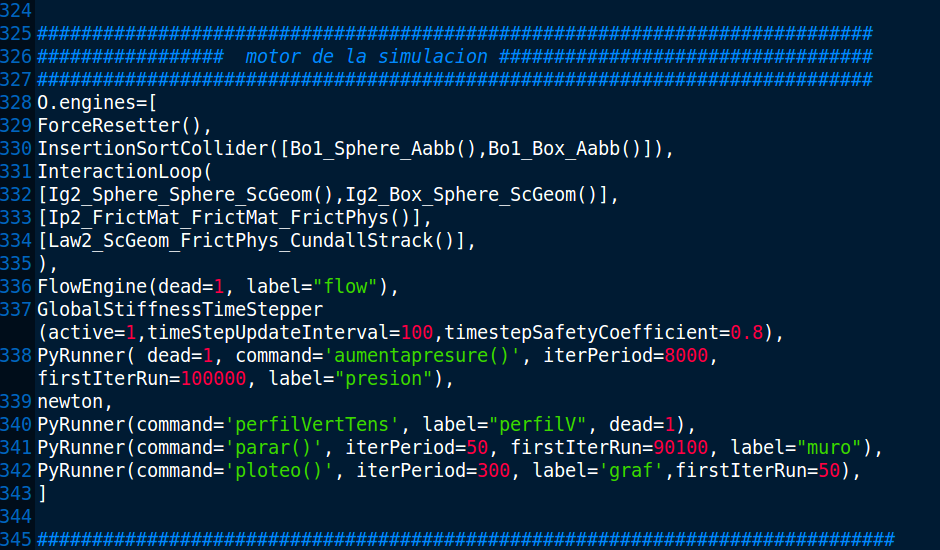
\includegraphics[width=\textwidth]{Anexo5/motor.png}
\caption{Motor de la simulaci\'on.}
\label{fig:motor}
\end{figure}

\begin{figure}[htb]
\centering
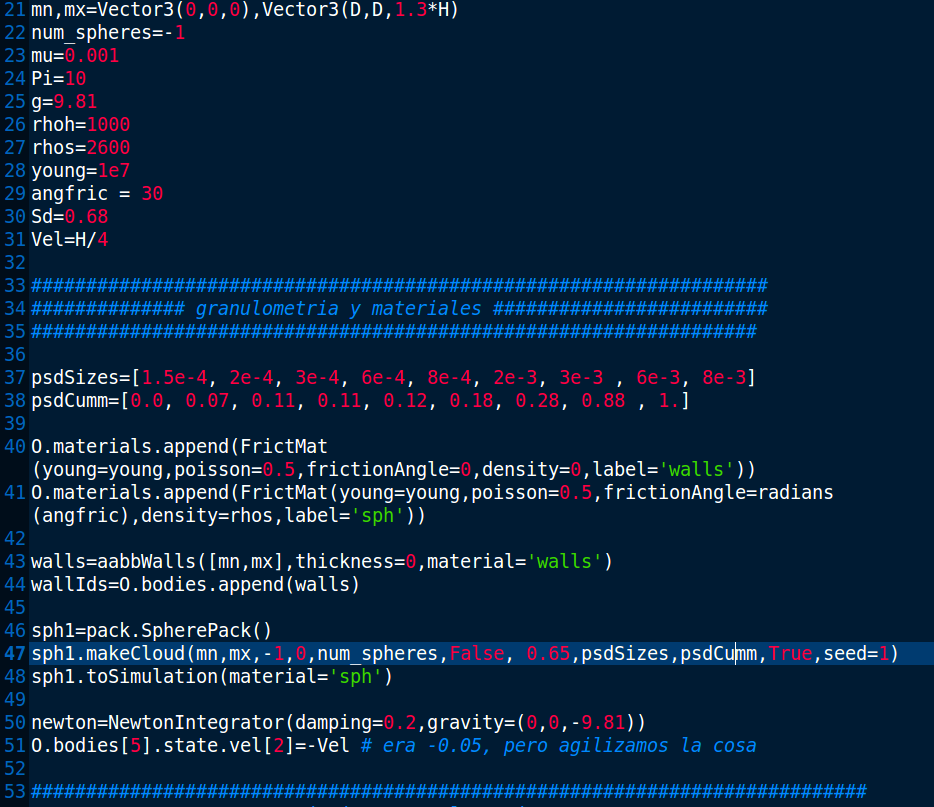
\includegraphics[width=\textwidth]{Anexo5/gran.png}
\caption{C\'odigo para crear una granulometr\'ia PSD.}
\label{fig:PSD15}
\end{figure}
